\chapter{基于WM算法的改进的多模式匹配算法}
\label{chap:WM}

\section{引言}
\label{sec:5_introduction}

WM \cite{Wu1994} 算法是Sun-Wu和Udi-Manber提出的一种快速多模式匹配算法,
该算法吸收了BM算法中的“坏字符”跳跃策略,并将其扩展为“坏字符块”,使
其更加适用于多模式下的情形,并通过哈希技术实现了字符块之间的快速比对和
索引,算法在最优情况下的时间复杂度为$O(B*n/lsp)$(其中$B$为字符块的长
度,$n$为文本串长,$lsp$为最短模式串长)。随着模式集规模的增长,WM算法
在进行模式匹配时经常会遇到Hash链表过长的情况,并且需要遍历整个链表来完
成处理,导致算法效率降低。针对以上问题本文进行了相应的改进:通过动态选
取每个模式串的特征串,使特征串的后缀字符块在模式集中出现的频率尽可能少,
从而避免了模式串聚集于某些链表内造成链表过长的情况;通过为Hash表中每条
较长的哈希链构造相应的索引表来取代原算法的Prefix表,并通过在该索引表上
执行二分查找,使算法可以很快确定需要精确匹配的模式串,避免了对整个链表
的遍历。 本章内容组织如下:\ref{sec:5_WM}节简要介绍了WM算法的流
程。\ref{sec:5_DWM+}节介绍了对WM的两方面改
进:DWM和WM+。\ref{sec:5_experiment} 节进行了对比实
验。\ref{sec:5_conclusion}对本章进行总结。


\section{WM算法简介}
\label{sec:5_WM}

和大多数多模式匹配算法类似,WM算法的运行过程包括对模式集进行预处理,和
对文本进行匹配两个阶段:

\begin{enumerate}
\item \textbf{预处理}: 首先确定最短模式串长: $lsp=min\{|p_i||p_i \in
  P\}$, 然后对$\forall p_i \in P$ 选取
  $\overline{p_i} = p_i[1, \dots , lsp]$ 作为$p_i$的“特征串”。 最后根
  据这些提取出的特征串,建立起Shift表、Hash表、以及Prefix表。

  \begin{itemize}
  \item Shift表(跳转表):Shift表记录了由$\Sigma$中的字符构成的每一个
    长为$B$的字符块(block)(共有个$|\Sigma|^B$), 在所有特征串中出现的最右
    端位置与该特征串尾之间的距离。对任一个字符块$block_i$,通过一个哈希函
    数:$hash(block_i)=h_i, i=1 \sim |\Sigma|^B$,将其映射为一个整数$h_i$作
    为Shift表的索引(可以利用$block_i$自身的二进制编码所对应的十进制无符号
    整数,作为其哈希值,即可实现字符块到正整数的一一映射)。若$block_i$不
    在任何特征串中,则$Shift[h_i]=lsp-B+1$;假设$block_i$在某个特征串中的终止
    位置为$q$,且在其他特征串中的终止位置不大于$q$,则$Shift[h_i] = lsp-q$。
  \item Hash表(哈希表):Hash表的每一项连接了一个模式串链表(简称哈希
    链),该链表中所有模式串的特征串,其长为$B$的后缀具有同样的哈希
    值。Hash表的大小与Shift表相同,并用相同的哈希值作索引。
  \item Prefix表(前缀表):Prefix表的构造与Hash表类似,每一项也连接着
    一个模式串链表,该链表中所有模式串具有相同的前缀。前缀通常取2个字
    符。
  \end{itemize}

\item \textbf{匹配}: 一旦Shift表、Hash表、以及Prefix表被建立完毕,便可
  以用其进行多模式匹配,包括以下几个步骤:

  \begin{itemize}
  \item 初始化:选取文本串$T$中前$lsp$个字符构成的子串,作为当前的“匹
    配窗口”,令$i=lsp$.
  \item 步骤 1. 若$i \leq |T|$, 计算当前匹配窗口长为B的后缀的哈希
    值:$h_s=hash(T[i-B+1, \dots, i])$; 否则,算法结束。
  \item 步骤 2. 若 $Shift[h_s] \neq 0$, 令 $i=i+Shift[h_s]$, 转到步
    骤1; 否则, 转到步骤 3。
  \item 步骤 3. 计算当前匹配窗口长为2的前缀的哈希值:
    $h_p=hash(T[i-lsp+1, i-lsp+2])$。通过查找Prefix表,对
    $\forall p_i \in Hash[h_s]$, 若
    $hash(p_i[1,2])=h_p$,则将$p_i$与$T$的相应部分进行精确匹配,若匹配
    成功则输出结果。
  \item 令 $i=i+1$, 转到步骤 1。
  \end{itemize}
\end{enumerate}

由以上分析可知,WM算法存在两个固有缺陷:(1) 算法性能受最短模式串
长$lsp$的影响较大。由Shift表的构造可知,算法每次的跳跃距离不能超过最短
模式串长,当模式集中包含极短模式串时,每次的跳跃距离将非常有限。(2) 当
模式串规模增大时,Shift表的作用亦会减小,同时会产生模式聚集现象,使
得Hash表中的某些链表过长,导致需要精确匹配的模式串大大增加,严重影响算
法性能。针对以上问题也有不少研究者进行了改进:刘卫国等
人 \cite{Liu2011} 等人采用双哈希策略,提出了DHSWM算法,避免了在大规模模
式集的情况下查找过长的模式串链表。Choi等人\cite{Choi2011} 通过增加最短
模式串长度,提出了L+1-MWM算法,使得Shift表的平均跳跃距离增加。张鑫等
人 \cite{Zhang2003},通过引入“精确的不良字符转移”和“弱化良好后缀转
移”的策略,增加了匹配成功时的跳跃距
离。Yang等人\cite{Hong2007} 结合QS算法 \cite{Sunday1990} 的思想提出
了QWM算法,增大了算法的平均跳跃距离。董迎亮等人 \cite{Dong2011},在原算
法的基础上,又引入了模式串尾字符块的过滤机制,进一步过滤掉无用模式
串。Zhang \cite{Zhang2009b} 等人在查找时通过判断Prefix链表中的模式串是
否在Hash表地址范围内,来提高哈希链表查找速度。Zhenlong Yuan
\cite{Yuan2013} 等人利用4字节字符块和两段哈希技术提出了TFD算法,能有效
解决过滤大规模URL模式串的问题。Xunxun Chen \cite{Chen2005} 等人将AC算法
的思想与WM算法相结合,提出了Tuned WM算法,增加了WM算法的平均跳转距离。


\section{基于WM的改进算法}
\label{sec:5_DWM+}

本节主要从调整Hash表中哈希链的长度分布和加速对哈希链的搜索两方面,
对WM算法进行改进。这两种方法完全依靠模式集自身的信息,不需要任何额外信
息,且非常易于实现,下面介绍具体方案。

\subsection{动态选择特征串(DWM)}
\label{sec:5_DWM
}

原始的WM算法总是选择模式串长为$lsp$的前缀作为其特征串,然而这种选择方法
没有充分考虑模式串自身的特点,在某些情况下会使算法陷入严重的瓶颈。例如,
给定模式集:
$P=\{p_1:abden,\, p_2:abduct,\, p_3:abd,\, p_4=abduce,\,
p_5=abducent\}$。
令$B=2$,则按照原算法的选择方式,所有模式串的特征串都将是$abd$,其特征
串长为2的后缀($bd$)自然也都相同,这样所有的模式串都将被分配到Hash表的同
一个表项$bd$中,如图 \ref{fig:WM_hash_table1} 所示。


\begin{figure}[H]
  \centering
  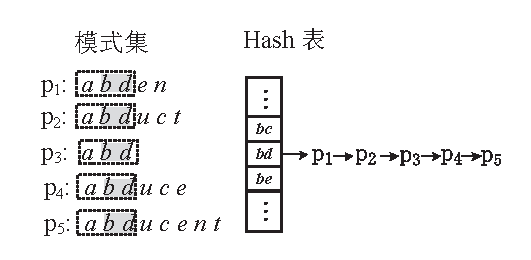
\includegraphics[height=4cm ,width=10cm]{figures/5_WM/hash_table1.eps}
  \caption{WM算法为模式集构建的Hash表。}
  \label{fig:WM_hash_table1}
\end{figure}

这将导致在匹配过程中只要遇到字符块$bd$都需要遍历所有模式串,严重影响了
算法性能。实验证实,当模式集规模增大时,该问题愈加明显。亦有学者对此进
行了研究,主要集中于如何选择模式串的特征串,例如,文献\cite{}提出了一种
基于文本信息的特征串选择策略,但该方法需要文本的先验知识,而这往往是未
知的;文献\cite{Tan2011} 给出了一种基于机器学习的特征串选择方法,但其实
现起来较为复杂,当模式集变化较快时,算法的预处理时间较长。下面给出一种
仅仅依赖于模式集自身信息,且易于实现的特征串选择方法:

首先,对所有长为$B$的字符块 $block_i, i=1 \sim |\Sigma|^B$, 计算其在给
定模式集中的出现频率即: $freq(block_i)=|P'|$, $P' \subseteq
P$且对$\forall p \in P'$, $block_i$都是$p$的子串。 然后在每个模式串中选
择出现频率最少的字符块并以此确定其特征串,这样选择出的特征串能够有效地
刻画模式串自身的特性,具有较强的区分度,可以有效地克服原算法存在的问题。
例如,对于上述的模式集,我们事先统计出每个字符块在该模式集中的出现频率,
如表 \ref{tab:block_freq} 所示(未出现的字块频率均为0):\\


\begin{table}[!htbp]
\centering
\vspace{-8pt}
\topcaption{所有长为2的字符块在给定模式集中的出现频率}
\begin{tabular}{|c|c|c|c|c|c|c|c|c|c|c|} \hline
  ... & $ab$ & $bd$ & $du$ & $uc$ & $ce$ &  $en$ & $nt$ & $ct$ & $de$ & ... \\\hline
  ... & 5 & 5 & 3 & 3 & 2 & 2 & 1 & 1 & 1 & ... \\
  \hline
  \end{tabular}
  \label{tab:block_freq}
\end{table}


对于 $p_1=abden$,可供选择的特征串为:$abd$, $bde$, $den$,由于在$bd$,
$de$,
$en$中$de$的出现频率最低,所以选择$bde$作为$p_1$的特征
串:$\overline{p_1}=bde$。类似地,我们
有:$\overline{p_2}=uct$,$\overline{p_3}=abd$,$\overline{p_4}=uce$,
$\overline{p_5}=ent$。用这样的特征串构造出的Hash表如
图\ref{fig:WM_hash_table2}所示:

\begin{figure}[!h]
  \centering
  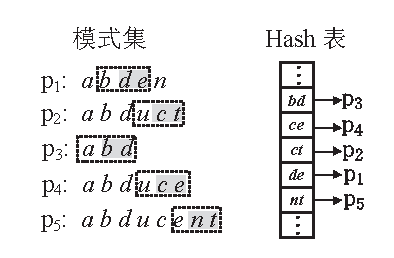
\includegraphics[height=4cm ,width=8cm]{figures/5_WM/hash_table2.eps}
  \caption{DWM算法为模式集构建的Hash表。}
  \label{fig:WM_hash_table2}
\end{figure}

这种选择策略避免了由于模式串的聚集而造成哈希链过长的情况,并且在匹配时
遇到某个字符块将会搜索最有可能匹配该字块的模式串,减少了搜索范围,因为
我们在选择每个模式串的特征串时,都是选择其(相对)最具代表性的部分作为
特征串的。下面是具体算法:

\begin{algorithm}
  \caption{计算字符块的出现频率(步骤 1)}
  \label{alg:block_freq}
  \begin{algorithmic}[1]
    \REQUIRE ~~\\
    模式集 $P$。 \\
    \ENSURE ~~\\
    每个长为$B$的字符块在 $P$中模式的出现频率。\\
    \STATE
    \STATE 创建长为$|\Sigma|^B$的数组$freq$(并将其元素初始化为0),用来记录字符块
    的出现频率。
    \STATE 创建长为$|\Sigma|^B$的数组$tag$,用来标记模式串中的字符块是
    否已经出现过。
    \STATE 变量$j$用于标记模式中字符块的起始位置。
    \STATE $block_{ij}$表示模式串$p_i$中,起始于位置$j$的字符块。
    \FOR{ $\forall p_i \in P$}
    \STATE 将$tag$数组清零。
    \FOR{$p_i$中每一个长为$B$的字符块 $block_{ij}$, $j=1 \sim |p_i|-B+1$}
    \IF{$tab[block_{ij}]\neq0$}
    \STATE $freq[block_{ij}] \leftarrow freq[block_{ij}]+1$
    \STATE $tab[block_{ij}]=1$
    \ENDIF
    \ENDFOR
    \ENDFOR
    \STATE
    \RETURN $freq$ 数组。
  \end{algorithmic}
\end{algorithm}


注意,如果一个字符块在某个模式串中出现多次,只按出现一次算,因此在扫描
每个模式串时,需要一个标记表$tag$,来记录某个字符块是否在该模式串中出现
过。对于模式串$p_i$,其包含的长为$B$的字符块数为$|p_i|-B+1$,而对每个模
式串,算法将扫描其中所有长为$B$的字符块,若模式集包含$k$个模式串,则总
的扫描次数将为:$\sum_{i=1}^{k}(|p_i|-B+1)$,因此,步骤 1的时间复杂度
为:$O(模式串长之和)$.

\begin{algorithm}
  \caption{选择特征串(步骤 2)}
  \label{alg:choose_signature}
  \begin{algorithmic}[1]
    \REQUIRE ~~\\
    模式集 $P$, 字符块频率表 $ferq$。 \\
    \ENSURE ~~\\
    每个模式串的特征串。\\
    \STATE
    \STATE $lsp \leftarrow$ 最短模式串长。
    \STATE 变量 $min\_block$ 代表当前模式串中出现频率最少的字符块。
    \STATE 
    \FOR{ $\forall p_i \in P$}
    \STATE $j \leftarrow lsp-B+1$
    \STATE $min\_block \leftarrow block_{ij}$
    \FOR{$p_i$中每个长为$B$的字符块: $block_{ij}$, $j=lsp-B+2 \sim |p_i|-B+1$}
    \IF{$freq[block_{ij}] < freq[min\_block]$}
    \STATE $min\_block \leftarrow block_{ij}$
    \STATE 选择以min\_block结尾,长为m的字符串作为的特征串。
    \ENDIF
    \ENDFOR
    \ENDFOR
  \end{algorithmic}
\end{algorithm}

对于任意模式串 $p_i$,其可供选择的特征串共有$|p_i|-lsp+1$个。对每个模
式串$p_i$,必须从起始位置为$lsp-B+1 \sim |p_i|-B+1$的这些字符块中,选
择频率最小的一个作为特征串的后缀,而不是从头开始选取。若模式集包含$k$
个模式串,则步骤 2需要扫描的字符块总数为$\sum_{i=1}^{k}(|p_i|-lsp+1)$,
因此其时间复杂度也为:O(模式串长之和)。综合以上两步,DWM预处理过程的时
间复杂度仅为:O(模式串长之和)。极低的时间复杂度和简单的实现过程保证了
DWM的可行性,其增加的额外的预处理开销微乎其微,因此完全适用于不断变化
的模式集。注意:DWM增加Hash表中哈希链的数目,导致了Shift表中值为0的项
增加,这会在一定程度上降低算法的跳转效率。但对于规模较小的模式集,性能
影响十分有限,且可以通过下一节将要介绍的哈希链加速技术来弥补;而当模式
集规模较大时,无论是原算法还是改进算法,Shfit表中几乎所有项都将为0,算
法跳转可能性大大降低,此时,算法的效率将主要取决于Hash表的表项分布,所
以对于较大规模的模式集,DWM明显地提升了原算法的性能,后面的实验证明了
该结论。

\subsection{加速哈希链的搜索(WM+)}
\label{sec:5_WM+}

原算法所构造的Prefix表效率很低,在匹配时,一旦遇到$Shift[block]=0$的情
形,要遍历整个$Hash[block]$所对应的链表来确定需要精确匹配的模式串,若链
表长度为$N$,其时间复杂度为$O(N)$,当哈希链很长且被频繁命中时,将会严重
影响算法性能。如果在构建哈希链时,事先按照特征串前缀哈希值的大小对模式
串进行排序,并为每条较长的链表建立相应的索引表,则在命中该哈希链时,只
需在索引表上进行二分查找,便可在$O(logn)$时间内找到需要进行精确匹配的模
式串,$n$为索引表的大小。索引表完全取代了原算法Prefix表的功能,且提高了
算法效率。

\begin{figure}[H]
  \centering
  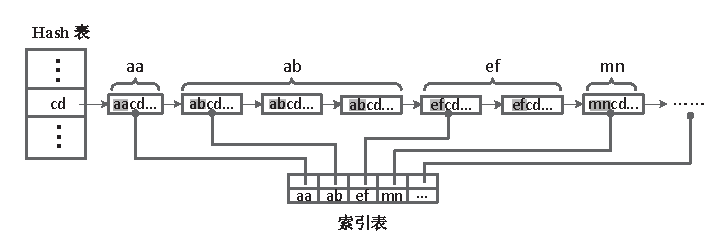
\includegraphics[height=5cm ,width=12cm]{figures/5_WM/index_table.eps}
  \caption{为长哈希链建立索引表结构。}
  \label{fig:WM_index}
\end{figure}

图\ref{fig:WM_index}显示了Hash表中字符块$cd$的哈希链表及为其建立的索引
表,假设$B=2$,前缀也取2个字符,最短模式串长$lsp=4$,对每个模式串(按照
原算法)取前4个字符作为其特征串。该哈希链中的所有模式串,按照其前缀哈希
值由小到大进行排序,这样前缀相同的模式串会被连续地排列在一起,依次遍历
该哈希链,对于每一个不同的前缀为其在索引表中建立一项,并将其指向哈希链
中具有该前缀的第一个模式串,这样构建的索引表也是有序的,通过它可以实现
对哈希链的快速搜索。例如,假设当前文本串的匹配窗口的后缀为$cd$,前缀
为$ef$,则无需遍历整个哈希链来寻找前缀为$ef$的模式串,只需要在索引表上
进行二分查找,便可迅速确定前缀为$ef$的模式串在哈希链中的起始位置,对从
起始位置开始的模式串依次进行精确匹配,直到遇到前缀不为$ef$的模式串为止
(无须记录其终止位置)。下面是建立索引表的算法(假设每条链表已经排好
序):

\begin{algorithm}
  \caption{为较长的哈希链表构建索引表}
  \label{alg:build_index}
  \begin{algorithmic}[1]
    \REQUIRE ~~\\
    Hash表。 \\
    \ENSURE ~~\\
    为其中较长链表构建索引表。\\
    \STATE
    \STATE 变量$pre\_prefix$表示前一个特征串的前缀。
    \STATE 变量$cur\_prefix(p)$表示当前模式串$p$的特征串的前缀。
    \STATE 
    \FOR{Hash表上的每条非空链表}
    \IF {该链表长度 > 特定阈值}
    \FOR{该链表上的每个模式串$p$}
    \IF{$cur\_prefix(p) \neq pre\_prefix$}
    \STATE 为$p$在索引表中新建一项,并指向$p$
    \STATE $old\_prefix \leftarrow cur\_prefix(p)$
    \ENDIF
    \ENDFOR
    \ENDIF
    \ENDFOR
  \end{algorithmic}
\end{algorithm}

并不需要对所有哈希链都建立索引表,因为对于很短的链表,调用二分查找的开
销要比直接遍历的开销更大,所以只有当哈希链的长度达到一定阈值时,才需建
立索引表,该阈值与具体的模式串集有关(通常设为10)。该算法只需对每条哈
希链扫描一遍,即可建立起相应的索引表,因此为整个Hash表建立索引表,最多
需要扫描所有哈希链一遍,这等价于扫描所有模式串一遍,因此建立索引表的时
间复杂度为$O(|P|)$, 即模式集规模;空间复杂度方面,原算法的Prefix表需
要$O(|P|)$的空间,而由上述可知,只有对较长的哈希链才为其建立索引表,且
索引表的长度远小于哈希链的长度,因此全部索引表所占的空间将远小
于$O(|P|)$。


\section{实验结果}
\label{sec:5_experiment}

由于两种改进方案的出发点不同,为了定量分析DWM和WM+对原算法的影响,将分
别对其进行了测试。首先测试了各算法在不同规模模式集下的性能;另外,由
于WM算法受最小模式串长的影响很大,也将测试最小模式串长对各算法的影响。

实验在一台笔记本电脑是进行, 软硬件配置如下: Intel Core i7-2630QM
2.00GHz CPU, 8GB RAM, 500GB 磁盘。 操作系统为 Ubuntu 14.04-64bit。  所
有算法由 C/C++ 实现, 由 \emph{gcc} 4.8.2 编译 (-O3)。

\subsection{模式集规模对算法的影响}
\label{sec:5_exp_1}

文本数据采用10M普通英文文本(约1000万字符),从文本中分别随机抽取1000,
2000, ...., 50000数量的模式串构成模式集。在每个模式集中,串长范围:$5
\sim 20$,平均串长:12.3,串长标准差:4.6。


\begin{figure}[H]
  \centering
  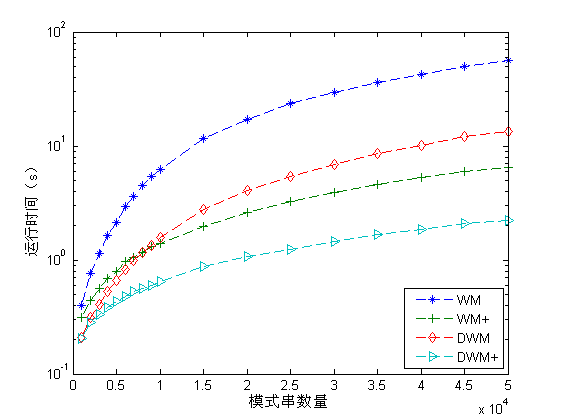
\includegraphics[height=7.5cm ,width=9.5cm]{figures/5_WM/WM_exp1.png}
  \caption{各算法在不同规模模式集下的运行时间对比(取对数)。}
  \label{fig:WM_exp1}
\end{figure}

\begin{figure}[H]
  \centering
  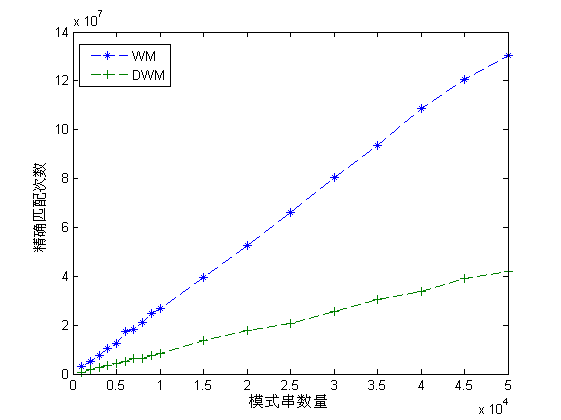
\includegraphics[height=7.5cm ,width=9.5cm]{figures/5_WM/WM_exp2.png}
  \caption{WM与DWM在不同规模模式集下的精确匹配次数对比。}
  \label{fig:WM_exp2}
\end{figure}



由实验结果可知,随着模式集规模$|P|$的增加,原算法的效率会逐渐降低,这主
要是由随着模式串数量的增长,文本中的$B$位字符块,几乎都会命中某些模式串
(的特征串),使跳转的可能性大大减小,此时算法的性能主要取决于Hash表的
结构(链长分布)和对哈希链的搜索速度。由图 \ref{fig:WM_exp1}可知,无论
是改变Hash表的链长分布(DWM),还是加速哈希链的搜索(WM+)都能大幅提升
算法的性能:改变链长分布可以减少算法在运行过程中执行精确匹配的次数;加
速对哈希链的搜索则能够迅速找到需要精确匹配的模式串。特别地,由
图 \ref{fig:WM_exp2}可知,DWM执行精确匹配操作的次数仅为WM的1/3,这是由
于在本例中,模式集是从文本中抽取得到,可将其视为文本的一个小样本,因此
模式集也能部分反映文本的特点:对于一个长为B的字符块,它在模式集中出现频
率的高低,与它在文本中大致相同,并且随着模式集的增长这种反映将更加准确。
这样,在Hash表中,由模式集中的高频字符块对应的哈希链,在扫描文本串时会
被更加频繁地命中,类似地,低频字符块对应的哈希链,在匹配时被命中的概率
相对较低。因此,DWM实际上是将会被高频率命中的哈希链中的模式串,转移到低
频哈希链中,这样减少了(高频)哈希链的长度,需要精确匹配的模式串数也随
之减少。从实际运行时间来看,当$|P|<10^4$,DWM效果较好;当$|P| \geq
10^4$,WM+效果较好,因为随着模式串数量的增加,哈希链的平均长度会随之增
加,因此加快对哈希链的搜索就显得愈发重要。特别地,二者的结合DWM+,对于
任何规模的模式集都具有最好的性能。

\subsection{最短模式串长对算法的影响}
\label{sec:5_exp_2}

文本数据不变,以2, 3, 4, ...,
20分别作为最短模式串长($lsp$),从文本中随机抽取19个模式集,其中每个模
式集的模式数固定为10000,最大模式串长固定为20,即模式集之间只有最短模式
串长$lsp$不同。

\begin{figure}[H]
  \centering
  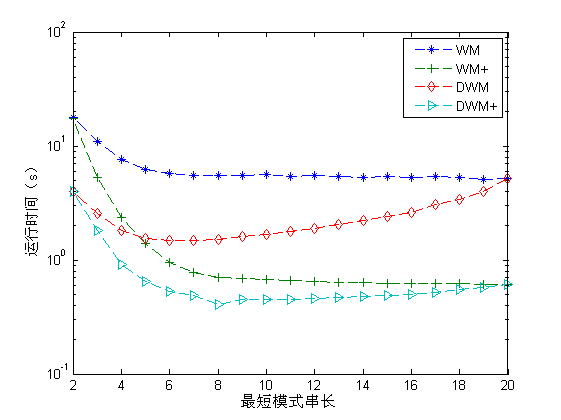
\includegraphics[height=7.5cm ,width=9.5cm]{figures/5_WM/WM_exp3.png}
  \caption{各算法在不同最短模式串长下的运行时间对比(取对数)。}
  \label{fig:WM_exp3}
\end{figure}

\begin{figure}[H]
  \centering
  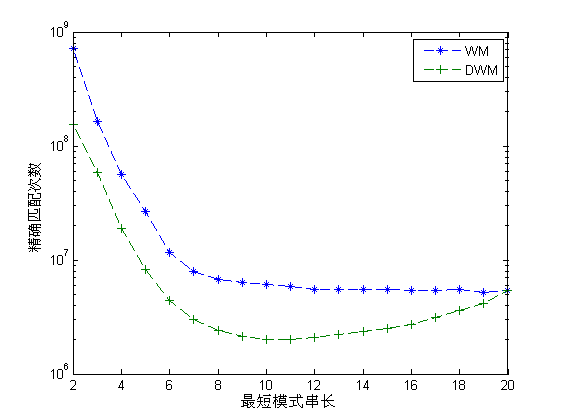
\includegraphics[height=7.5cm ,width=9.5cm]{figures/5_WM/WM_exp4.png}
  \caption{WM与DWM在不同最短模式串长下的精确匹配次数对比(取对数)}
  \label{fig:WM_exp4}
\end{figure}

由图\ref{fig:WM_exp3}可知,当$lsp<5$时原算法性能不佳,这主要是由于
当$lsp$较小时无法发挥坏字符块跳转的优势,因为Shift表的最大跳转距离不超
过$lsp-B+1$,在这种情形下算法的性能亦取决于Hash表的链长分布以及对哈希链
的查找速度。$lsp=2$是个极端情况,此时所有特征串长均为2且特征串的前缀及
后缀均为该特征串本身,这就导致一旦命中某条哈希链,该哈希链上的所有模式
串都需要进行精确匹配,WM+将失去作用。DWM算法明显改善了WM算法在$lsp$较小
时的性能,这是由于DWM合理的调整了Hash表的链长分布,将一些较长且会被频繁
遍历的哈希链上的模式分配到其他链表中,由图\ref{fig:WM_exp4}可知,
在$lsp=2$时,DWM的精确匹配次数仅为WM的1/5;当$2<lsp\leq 11$时,DWM的精
确匹配次数为WM的1/3,精确匹配次数的减少直接降低了算法的运行时间。从算法
的实际运行效果来看,当$lsp<5$时,DWM优于WM+;当$lsp \geq 5$时,WM+更有
优势;当$lsp > 7$时,DWM对原算法的性能提升逐渐减弱(依然优于),这是因
为随着$lsp$的增加,可供选择的特征串将越来越少(对于任意模式串$p$,其可
供选择的特征串数为:$|p|-lsp+1$),当$lsp=20$(即所有模式串长均为20)
时,DWM退化成WM,类似地DWM+退化成WM+。我们又一次看到,两种方法的结
合DWM+在任何情况下都具有最优性能。

\section{本章小节}
\label{sec:5_conclusion}

本文主要针对WM算法做了两点改进:(1) 通过寻找每个模式串中出现频率最少的
字符块来确定该模式的特征串,以这样的特征串来构造Hash表避免了出现过长哈
希链的情况,并可将频繁遍历的哈希链中的模式串转移到其它哈希链中,减少了
程序运行中精确匹配的次数,该方法对于包含较短模式的模式集以及模式集和文
本相互有关联的情况,效果尤为明显;(2) 通过为较长的哈希链建立一个索引表,
并通过在该索引表上的二分查找,算法可以在极短的时间内找到需要精确匹配的
模式串,避免了对整条哈希链的遍历,随着模式集规模的增加该方法效果愈加明
显。特别地,两种改进方案的结合,在任何情况下性能都是最优的。
